\definecolor{acmBlue}{HTML}{4477AA}
\definecolor{acmTeal}{HTML}{228833}
\definecolor{acmSand}{HTML}{EE7733}
\definecolor{acmGrid}{HTML}{D9DDE2}
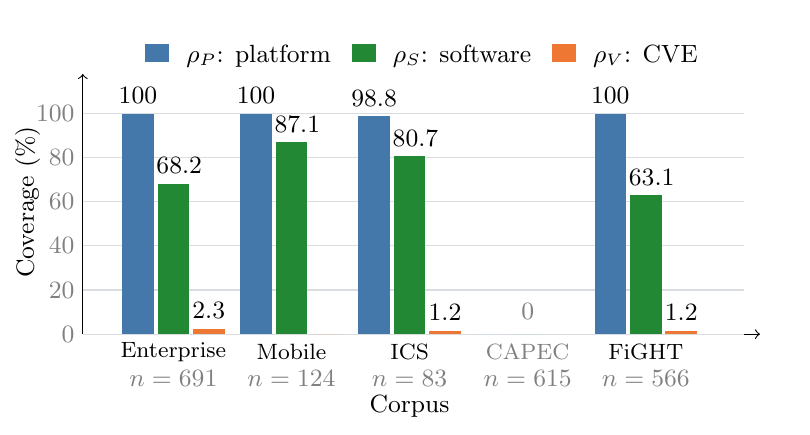
\begin{tikzpicture}[x=0.50cm,y=0.028cm,font=\small]
  \path[use as bounding box] (-1.40,-33.0) rectangle (17.75,139.0);
  \draw[->] (0,0) -- (17.2,0);
  \draw[->] (0,0) -- (0,118);
  \node[rotate=90,font=\small] at (-1.4,60) {Coverage (\%)};
  \foreach \yy in {0,20,40,60,80,100} {
    \draw[acmGrid] (0,\yy) -- (16.8,\yy);
    \node[anchor=east,font=\small,text=gray,inner xsep=0.8pt,inner ysep=0.2pt] at (-0.14,\yy) {\yy};
  }
  \fill[acmBlue]   (1.0,0) rectangle (1.8,100.0);
  \fill[acmTeal]   (1.9,0) rectangle (2.7,68.2);
  \fill[acmSand]   (2.8,0) rectangle (3.6,2.3);
  \node[above,font=\small] at (1.4,100.0) {100};
  \node[above,font=\small] at (2.45,68.2) {68.2};
  \node[above,font=\small] at (3.2,2.70) {2.3};
  \fill[acmBlue]   (4.0,0) rectangle (4.8,100.0);
  \fill[acmTeal]   (4.9,0) rectangle (5.7,87.1);
  \fill[acmSand]   (5.8,0) rectangle (6.6,0.0);
  \node[above,font=\small] at (4.4,100.0) {100};
  \node[above,font=\small] at (5.45,87.1) {87.1};
  \fill[acmBlue]   (7.0,0) rectangle (7.8,98.8);
  \fill[acmTeal]   (7.9,0) rectangle (8.7,80.7);
  \fill[acmSand]   (8.8,0) rectangle (9.6,1.2);
  \node[above,font=\small] at (7.4,98.8) {98.8};
  \node[above,font=\small] at (8.45,80.7) {80.7};
  \node[above,font=\small] at (9.2,1.70) {1.2};
  \fill[acmBlue!40]   (10.0,0) rectangle (10.8,0.0);
  \fill[acmTeal!40]   (10.9,0) rectangle (11.7,0.0);
  \fill[acmSand!40]   (11.8,0) rectangle (12.6,0.0);
  \node[above,font=\small,text=gray] at (11.3,2) {0};
  \fill[acmBlue]   (13.0,0) rectangle (13.8,100.0);
  \fill[acmTeal]   (13.9,0) rectangle (14.7,63.1);
  \fill[acmSand]   (14.8,0) rectangle (15.6,1.2);
  \node[above,font=\small] at (13.4,100.0) {100};
  \node[above,font=\small] at (14.45,63.1) {63.1};
  \node[above,font=\small] at (15.2,1.70) {1.2};
  \node[font=\footnotesize] at (2.3,-8) {Enterprise};
  \node[font=\footnotesize] at (5.3,-8) {Mobile};
  \node[font=\footnotesize] at (8.3,-8) {ICS};
  \node[font=\footnotesize,text=gray] at (11.3,-8) {CAPEC};
  \node[font=\footnotesize] at (14.3,-8) {FiGHT};
  \node[below,font=\small,text=gray] at (2.3,-12) {$n=691$};
  \node[below,font=\small,text=gray] at (5.3,-12) {$n=124$};
  \node[below,font=\small,text=gray] at (8.3,-12) {$n=83$};
  \node[below,font=\small,text=gray] at (11.3,-12) {$n=615$};
  \node[below,font=\small,text=gray] at (14.3,-12) {$n=566$};
  \node[font=\small,text=black] at (8.3,-33.0) {Corpus};
  \node[anchor=north,fill=white,fill opacity=0.95,text opacity=1,inner sep=2.2pt] at (8.6,136.0) {
    \begin{tabular}{@{}c@{\hspace{0.8em}}c@{\hspace{0.8em}}c@{}}
      \textcolor{acmBlue}{\rule{0.95em}{0.72em}}\ \ $\rho_P$: platform &
      \textcolor{acmTeal}{\rule{0.95em}{0.72em}}\ \ $\rho_S$: software &
      \textcolor{acmSand}{\rule{0.95em}{0.72em}}\ \ $\rho_V$: CVE
    \end{tabular}
  };
\end{tikzpicture}
